\documentclass[twocolumn]{article}

% Feel free to add more packages
\usepackage{float, amsmath, amssymb, mathtools}
\usepackage{graphicx, caption, color}
\usepackage{tabularx, fullpage}
%\usepackage{kotex}
%\usepackage{multicol}
\setlength{\columnsep}{1cm}
\usepackage{comment, cite, wrapfig}
\usepackage[utf8]{inputenc}
\usepackage[hidelinks]{hyperref}
\usepackage{courier}
\usepackage{listings}
%\usepackage{geometry}
\hypersetup{breaklinks=true}
\urlstyle{same}

\newcommand{\red}[1]{{\bf \color{red}#1}}
\newcommand{\blue}[1]{{\bf \color{blue}#1}}
\newcommand{\cut}[1]{}


\begin{document}

\title{Natural Language Interface for Relational Database\\	
	\small{Final Report}\footnote{The github repository for this project is \url{https://github.com/DukeNLIDB/NLIDB}}}

%Authors in alphabetical order of last names
\author{Yilin Gao \\
	\small \texttt{yilin.gao@duke.edu} \and 
	Keping Wang \\
	\small \texttt{kw238@duke.edu} \and 
	Chengkang Xu \\
	\small \texttt{cx33@duke.edu} }
	
\date{\today}
\maketitle

%%%================================================================%%%
\section{Introduction}\label{sec:introduction}

Writing SQL queries can be difficult, especially when it involves complex logic. As more and more non-expert users are accessing relational databases, it is very important to simplify their process of writing SQL queries. This project is going to build a Natural Language Interface for relational DataBases (NLIDB), closely following Li and Jagadish (2014)\cite{li2014}. NLIDB will be a tool for everyone to query data easily from relational databases.

Translating natural language into an SQL query isn't an easy job. Not only because of the ambiguity of natural language, but also that users may make mistakes in writing natural language input, such as mis-spelling. We want the users to feel at ease using our interface, not afraid of being mis-interpreted by the NLIDB, even if they cannot remember the exact names of the database column names. So we follow Li and Jagadish (2014)\cite{li2014} to use an interactive interface to let user make choices in several ambiguous phases of the translation.

The main components for translating a natural language to an SQL query are as follows:

\begin{enumerate}
  \item Parse the natural language input into a parse tree using dependency syntax parser.
  \item Map the nodes in the parse tree to SQL keywords, table names, column names, and values. Here users may choose the desired mapping from ranked options.
  \item Adjust the structure of the parse tree to make it follow the structure of an SQL query. Here users may choose the desired structure from ranked options.
  \item Translate the parse tree to an SQL query.
\end{enumerate}

In our project, we have accomplished all four steps, being able to carry out simple natural language queries (without join and complex nested conditions) with relatively high accuracy , and built an interactive graphical user interface (GUI) to communicate with users.

%%%================================================================%%%
\section{Related Work}

Early day NLIDB systems were usually based on small scale databases, which require a small set of supported queries. Their parsing mechanism could only support ad-hoc methods and rules. Thus, early work would produce ambiguity if the database is scalable and natural language queries are "open-domain". Moreover, without the help of machine learning, early NLIDB systems cannot update their parsing methods as they accumulate more data.\cite{QATutorial}

Our approach involves machine learning in parsing the natural language input into a parse tree. Then we adjust the structure of the parse tree to obey with the SQL syntax. Our approach can handle natural language input with more complicated structures than the simple key-word matching method. 

NLIDB here is a concrete application of the natural language QA systems.\cite{QATutorial} Currently, the mainstream approach for QA is the semantic parsing of questions. It can map natural language questions to logic forms or structured queries, and produce accurate answers when the query is complete and clear. However, the accuracy of answers will decrease if the input language is ambiguous, or if the logic relationship of the query is complicated. Due to our lack of training data, our NLIDB system cannot adopt the popular RNN (LSTM) for a direct and efficient translation. Still we are trying to allow for more input ambiguity and structural complexity by letting the users to choose the mappings and structures interactively.

%%%================================================================%%%
\section{Problem Definition}

For this NLIDB, we have to first develop a GUI, and design the structure of a parse tree. Then we need to develop parse tree node mapper, parse tree structure adjustor, and SQL query translator.

There are three main problems that we face. The first one is how to design the data structure for the parse tree. The second one is what algorithms to use for each phase of adjustment and translation. The last one is to specify the rules for different phases, such as what word should be mapped to the ``SELECT'' key word, and what rules should a legal parse tree follow before being translated to an SQL query.

%%%================================================================%%%
\section{Algorithms}

In the natural language parsing phase, we use the feature based pos-tagger\cite{toutanova2003feature} and the neural network dependency parser\cite{chen2014fast} from the Stanford NLP package.

In the node mapping phase, other than mapping words with hard coded rules, we compare words with table names, column names, and table values in the database, based on their word similarity scores. The similarity score is the maximum of two subscores. The first is lexical similarity (similarity in spelling), which is Jaccord coefficient here. The second is semantic similarity, for which we use WUP similarity\cite{wu1994verbs}. To compute WUP similarity, we have to do a breadth-first-search to find the lowest common ancestor of two words in the WordNet. The calculation of word similarity will be explained in detail in the next section.

In the tree structure adjusting phase, we reformulate the parse tree referring to and revising a specific algorithm provided by Li and Jagadish (2014)\cite{li2014}. The basic thought to traverse an exponentially large set of possible reformation of a tree is that, we revise the tree structure slightly step by step, by changing the space relationship among close nodes. More details on this algorithm will be provided in next section.

%%%================================================================%%%
\section{System Design}

\begin{figure*}[ht]
  \centering
  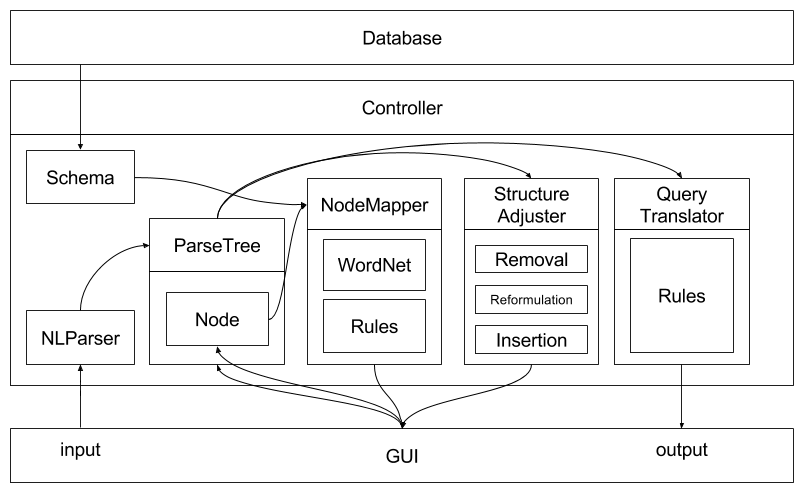
\includegraphics[width=0.8\linewidth]{figures/nlidb_system_diagram.png}
  \caption{System Diagram}
\end{figure*}

Our system is implemented in Java, using maven as the project management tool. Source codes are divided into three parts: model, control, and view. The model part takes care of how to realize major functions of the NLIDB, like parsing natural language, mapping nodes, adjusting parse tree structures, and translating the tree into SQL query. The controller wraps many models as attribute variables, and it takes charge of the interaction between database and the view (GUI). And the view part uses JavaFX to design a GUI. Figure 1 is a diagram of our system. 

Below we’ll introduce the design ideas on four major steps as explained before: natural language parsing, node mapping, parse tree reformulation, and SQL translation.

\subsection{Natural Language Parser}
We write the NLParser class to parse natural language from the user input in GUI to a dependency parse tree. The NLParser is just a wrapper of the Standford NLP pos-tagger and dependency syntax parser. A natural language sentence is first tagged with part-of-speech labels, and then parsed with dependency parser to a ParseTree.

A ParseTree consists of a set of nodes, connected by ``edges'' (parent-children relationship). Each node stores the natural language word and its corresponding SQL component (which will be assigned in the node mapping phase). A node also contains parent and children links pointing to other nodes in the ParseTree.

\subsection{Node Mapper}
Then we map each node into an SQL component. We iterate over the tree and map each node according to a certain node type in Figure 2, according to predefined rules provided by Li and Jagadish (2014)\cite{li2014}. There are 7 node types in total, and 5 of them (SN, ON, FN, QN, and LN) are defined with hard-coded mapping rules. For example, natural language words “return” and “Return” are mapped to an “SN” node with SQL value “SELECT”. A word will first be searched against these five node types. If there is no match, the search will go on to the remaining two types, NN and VN.

\begin{figure}[ht]
  \centering
  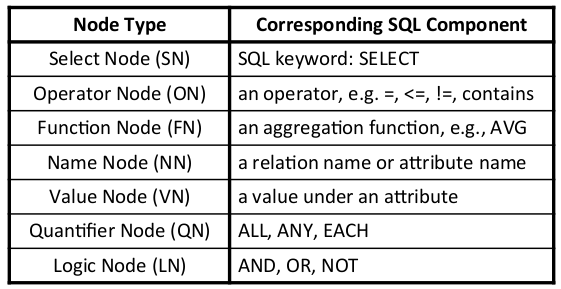
\includegraphics[width=0.9\linewidth]{figures/nodes_mapping_rules.png}
  \caption[caption for nodes mapping rules]{Nodes Mapping Rules\protect\footnotemark}
\end{figure}
\footnotetext{Taken from \cite{li2014}.}

The remaining two types, Name Node and Value Node, are decided by searching over the database for matching names or values. The matching of a word to names or values are decided by the word similarity score between two words.The word similarity score here is the maximum of semantic similarity and lexical similarity.

Semantic similarity is the WUP similarity\cite{wu1994verbs} function using WordNet. WordNet is a net of synonym sets (synsets) connected with semantic and lexical pointers. Two most important semantic pointers are hypernym and hyponym, which connect the synsets to the tree that we are interested here, as Figure 3. In Figure 3, the WUP similarity between $C1$ and $C2$ is:

$$ Sim_{WUP} = \frac{2*N3}{N1+N2+2*N3} $$

\begin{figure}[ht]
  \centering
  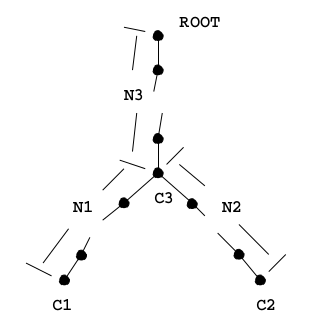
\includegraphics[width=0.7\linewidth]{figures/wordnet_tree.png}
  \caption[caption for wordnet tree]{WUP word similarity.\protect\footnotemark }
\end{figure}
\footnotetext{Taken from \cite{wu1994verbs}.}

One thing to note about WordNet is that each word can be in multiple synsets, and each synset can have multiple parents, so we use breadth-first-search to find the lowest of all possible common parents of two words.

For lexical similarity between two words, we use the Jaccard coefficient:

$$ J(A, B) = \frac{|A \cap B|}{|A \cup B|}$$

where $A$ and $B$ are the set of characters of the two words respectively. The Jaccard coefficient may not be as good for measuring the lexical similarity of two words (as edit distance), but it is currently still used because it is a measure in range (0,1), which makes it easily compared with the WUP semantic similarity.

To search over the database, we first visit the entire database, retrieve its schema, and store the Schema Graph as an attribute variable in the Controller class, so that each node mapping task don’t have to go through the slow database query. The Schema contains all table names, all column names, and some sample distinct values from each column (we use a sample of 10,000), such that they can be searched over to map Name Node or Value Node.

Once we have the word similarity scores of one word to names and values in database, we rank different mapping choices by their similarity score, and return the highest several choices to the GUI for the user to choose. Here we add another node type for the user to choose from, that is “UNKNOWN”, meaning that node doesn’t correspond to any meaningful SQL component. These meaningless nodes will be removed in later steps.

Figure 4 is an example of a parse tree with nodes mapped to SQL components. The left part is a parse tree, and the right part is the mappings of all its nodes.

\begin{figure}[ht]
  \centering
  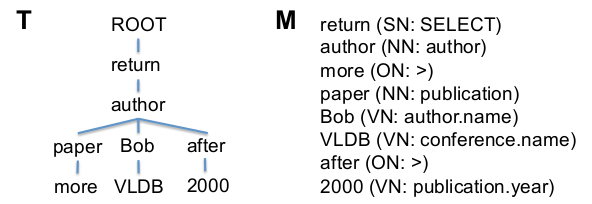
\includegraphics[width=0.9\linewidth]{figures/nodes_mapping_example.png}
  \caption[caption for nodes mapping example]{Node Mapping Example.\protect\footnotemark }
\end{figure}
\footnotetext{Taken from \cite{li2014}.}

\subsection{Parse Tree Reformulation}
Given a parse tree, there are several steps of reformulation.
\begin{enumerate}
	\item Remove mapped meaningless nodes in the tree.
	
	\item Merge the content of each Logic Node (LN) and Quantifier Node (QN) with its parent, and retain the node type of the parent node. This is to simplify future reformulation work.
	
	\item Use subtree move operations to edit the parse tree until it is syntactically valid according to the predefined grammar for a parse tree.
	
	The grammar works in this way:
	{\small 
	\begin{enumerate}
		\item Q $=>$ (SClause)(ComplexCindition)*
		
		\item SClause $=>$ SELECT $+$ GNP
		
		\item ComplexCondition $=>$ ON $+$ (LeftSubTree*RightSubTree)
		
		\item LeftSubTree $=>$ GNP
		
		\item RightSubTree $=>$ GNP $|$ VN $|$ FN
		
		\item GNP $=>$ (FN $+$ GNP) $|$ NP
		
		\item NP $=>$ NN $+$ (NN)*(Condition)*
		
		\item Condition $=>$ VN $|$ (ON $+$ VN)
	\end{enumerate}
	
	Note:
	All terminal nodes are predefined in this report.
	
	Q represents an entire query tree.
	
	+ represents a parent-child relationship.
	
	* represents a sibling relationship.
	
	One Query (Q) can must have one SClause and zero or more ComplexConditions.
	
	A ComplexCondition must have one ON, with a leftSubtree and a rightSubtree.
	
	An NP is: one NN (since an SQL query has to select at least one attribute), whose children are multiple NNs and Conditions. (All other selected attributes and conditions are stacked here to form a wide "NP" tree.)}
	
	The basic thought of the reformulation algorithm is that, in order to traversal all possible forms of the tree represented by a set of fixed nodes, which is an exponentially large set of trees, we need to reformulate the tree slightly step by step, discard those formulated trees with worse validity (according to our defined ``score'' for trees) than the original parse tree, and take the remaining formulated trees with better validity for future reformulation. This step is repeated recursively until there is no more new trees to be generated.
	
	The pseudocode for the algorithm works in this way:
	
	{\small 
	QueryTreeGen(ParseTree):
		
	results = $\emptyset$
	
	HashTable = $\emptyset$
	
	PriorityQueue.push(ParseTree)
	
	HashTable.add(ParseTree)
	
	\textbf{while} PriorityQueue $\neq\emptyset$ \textbf{do}:
	
	\hspace{1em} tree=PriorityQueue.pop()
	
	\hspace{1em} treeList=adjust(tree)
	
	\hspace{1em} \textbf{for all} tree'$\in$ treeList \textbf{do}:
	
	\hspace{2em} \textbf{if} tree' not exists in HashTable \textbf{and} tree'.edit $<$ t \textbf{then}:
	
	\hspace{3em} tree'.edit $=$ tree.edit $+1$
	
	\hspace{3em} HashTable.add(HashCode(tree'))
	
	\hspace{3em} \textbf{if} evaluate(tree') $\leq$ evaluate(tree) \textbf{then}:
	
	\hspace{4em} PriorityQueue.add(tree')
	
	\hspace{4em} results.add(tree')
	
	rank(results)
	
	\textbf{return} results
	}
	
	We use a hash table to store hash values for trees and make sure every tree is processed at most once. We set a parameter $t$ to limit the maximum number of edits approved. We use a function evaluate(tree) to compute the ``score'' of each tree, and if a newly generated tree has higher score than the original tree, we regard it as a bad tree and discard it directly. Otherwise, this tree is added into the priority queue, which stores trees with there ``score'' in ascending order, for future reformulation.
	
	We denote the ``score'' of each tree as the number of ``invalid'' nodes violating previous grammar. With more ``invalid'' nodes, a tree gets higher score and is more likely to be discarded right away. The complex rules to check if a nodes is ``invalid'' extend the recursive parse tree grammar and figure out the validity of nodes according to their word type. One basic rule is that, we only check the relationship between a node and its direct children to determine its validity. Take a Value Node (VN) for example, according to the grammar, it is invalid if and only if it has children.
	
	The most important part of this algorithm is to figure how to adjust a tree. In our adjustment algorithm, given a parse tree, we do the following 4 steps to each node and store the reformulated tree.
	
	\begin{itemize}
		\item Exchange this node with one of its children.
		\item If there are children, make one of its children its right sibling.
		\item If there are siblings, make one of its siblings its rightest children.
		\item If there are at least two children, switch the position of every pair of two children.
	\end{itemize}
	
	We can prove that this adjustment algorithm is complete and well adjusted to the nature of a parse tree.
\end{enumerate}

\subsection{Implicit Node}
The main idea of inserting implicit node into parse tree is to make sure that two nodes which are being mapped have corresponding schema in database. Assuming invalid nodes are removed from the tree properly, there shoud be a tree with at most three branches. The leftmost tree should contain select node (SN) and name node (NN). If a name node in the left tree does not have ancestor, then it is the core node of the left tree. If the type of core node in left tree is different from right tree, the real core node in right tree is deemed hidden, i.e. implicit. The implicit core node may cause unreasonable comparison between two variables of different types due to the change of semantic meaning. An example of implicit node: return all author who wrote more than 100 paper. In our previous process of the parse tree, the right subtree should contain only the number 100, which is a value node (VN). In order to make the tree semantically meaningful, nodes in left subtree are copied over to the right subtree.

After inserting name node based on the core node comparison, next step is to check the constrain for both core node. For example: if left core node has constrain of year greater than 2007 and area of "Database" , right core node should also have the same constrain. If right node does not conform to this constrain, then constrains nodes should be copied from the left subtree to right subtree. 

Our implementation of processing the implicit nodes insertion starts from the root of the tree. It checks if any nodes below select Node (SN) is missing in the middle tree. If there is, copy it over to the middle tree. Then repeat the same procedure to the middle tree and rightmost subtree. After the name node is copied over, it starts from the middle tree to check if there is any constrain missing in the rightmost tree. If there is, copy those over to the right tree. Finally,  if the root of subtree is an ON (operator node), and the first node connect to root in the subtree is a name node, there may be a function node missing. Our implementation tries to insert a function node in between to make the subtree semantically meaningful. 

\subsection{SQL Translation}
To do the SQL translation, first we create an SQLQuery object, with the structure "SELECT ... FROM ... WHERE ...;". Then we traverse over the tree and do the translation according to the grammar rules defined previously. For example, If we find a NameNode with value "article.title", then we add "article.title" to the SELECT part of the SQL Query, and add "article" to the "FROM" part of the query. If we find a ValueNode "1980" with value "article.year", then we add "article.year = 1980" to the WHERE clause, and add "article" to FROM clause. Here each component, SELECT, FROM, or WHERE, store the values in a set.

For now we can only handle "AND" logic for the WHERE clause. Parsing natural language into combinations of ANDs and ORs is itself a difficult task, which is not the focus of our project.

We also implemented the join of different tables. Whenever there are more than one tables in FROM clause, we know it's time for a join. We calculate the join path from the schema graph using breadth-first-search. We allow intermediate tables for joining two tables, and we find out the join key columns between every two tables using the following rule: a set of columns is a join key for two tables if it is the primary key of one table and contained but not the primary key of the other table.

Besides, we also layed out the basic framework for subquery blocks in complex conditions. A subquery block is obtained by starting a new SQL translation for a subtree. Each subquery block is added to the FROM clause of the main qu now we can only assume that all the columns columns in a subquery compose into a public key and are contained in other table(s) of the main query to allow join to happen appropriately.

%%%================================================================%%%
\section{Experiments}
The JavaFX application runs on JVM, and we’ve tested it on Mac OS X and Ubuntu 16.04 machine. We are using JDBC to connect to the PostgreSQL database of dblp, which we used in homework 1.

\begin{figure}[ht]
  \centering
  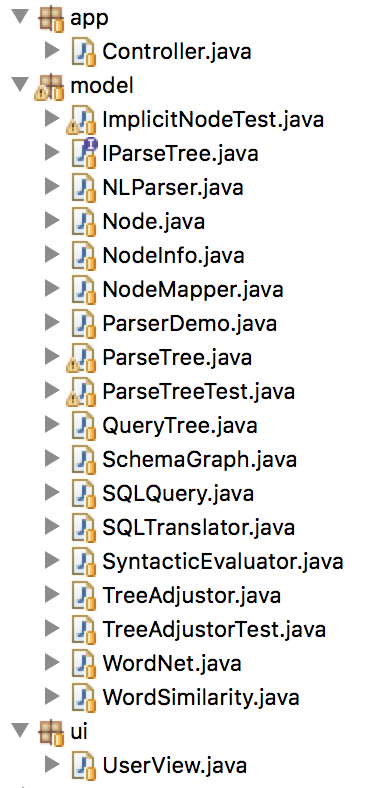
\includegraphics[width=0.8\linewidth]{figures/program_structure.png}
  \caption{Program Structure}
\end{figure}
  
Figure 5 is a detailed structure on programs in our project.

We have programmed a GUI in \texttt{UserView.java} and a connection between database and GUI in \texttt{Controller.java}. To realize natural language query, our first step in implementing the translation process is to parse the natural language into SQL keywords using a predefined natural language parser called Stanford NLP. The parsing process is written in \texttt{NLParser.java} and \texttt{ParserTree.java}. After we get the parser tree, we map each tree node (word in initial natural language input) to certain component of SQL and database. The mapping is written in \texttt{NodeMapper.java}. Reformulating parse tree and inserting implicit nodes and related functions are written in \texttt{ParseTree.java}, \texttt{TreeAdjustor.java} and \texttt{SyntacticEvaluator.java}. Translating to SQL is written in \texttt{SQLTranslator.java} and \texttt{SQLQuery}.

\begin{figure}
	\centering
	\begin{minipage}{0.45\textwidth}
		\centering
		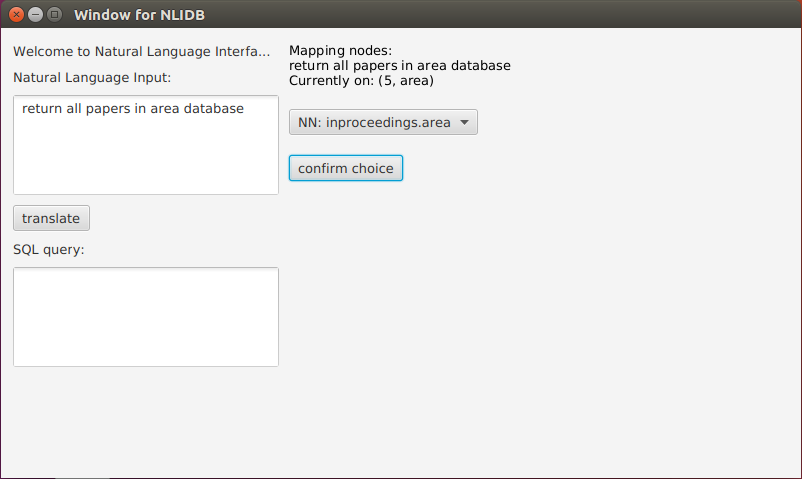
\includegraphics[width=0.9\textwidth]{figures/gui_nodes_mapping.png} % first figure itself
		\caption{GUI during Node Mapping}
	\end{minipage}\hfill
	\begin{minipage}{0.45\textwidth}
		\centering
		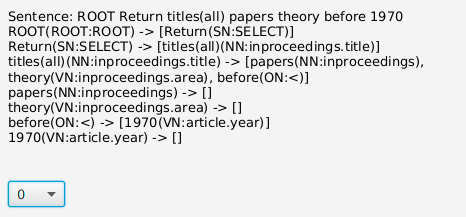
\includegraphics[width=0.9\textwidth]{figures/gui_tree_adjustor1.png} % second figure itself
		\caption{GUI after Tree Reformulation}
	\end{minipage}\hfill
	\begin{minipage}{0.45\textwidth}
		\centering
		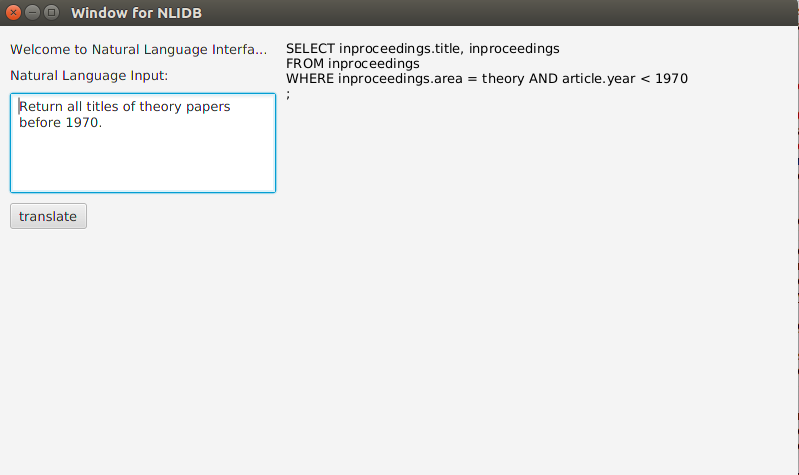
\includegraphics[width=0.9\textwidth]{figures/gui_translation.png} % second figure itself
		\caption{GUI after SQL Translation}
	\end{minipage}
\end{figure}

Figure 6 is a screenshot of our application during the nodes mapping stage. The upper left part is where the user input comes. The bottom left part is supposed to be the translated SQL query (which hasn’t been completed). The upper left part shows the current information on nodes mapping. The choice box showing “NN: inproceedings.title” contains a drop down list of node types and values for the user to choose from. Once the user confirms the choice by pressing the “confirm choice” button, the app will go on to map the next word. The mapping choices will only be shown to the user if the word doesn’t match with the five predefined node types.

Figure 7 is a screenshot of our application after the tree reformulation stage, showing the first parse tree out of 3 choices. The user will go through 3 choices and choose their most ideal tree structure. The tree structure is printed out firstly in preorder traversal, later in parent-children relationship. We can notice that the first choice is almost same as the correct parse tree structure.

Figure 8 is a screenshot of our application after the SQL translation stage, translated the previous selected parse tree into SQL.

For the node mapper, we’ve only defined very limited number of explicit rules for nodes mapping. There are only a few predefined keywords, such as return, equals, all, etc (thus limited SQL query functions as well). The nodes mapping for name nodes and value nodes doesn’t work perfectly well, maybe in the future we will try some more sensible measures of word similarity. But it is ok for now, since the users can almost always find the right name node or value node from the multiple choices. 

In the parse tree reformulation phase, we have correctly defined the grammar rules for checking transformed trees and implemented the algorithm. At first, because the size of output was so large, it was really hard for the user to pick up an ideal tree from a limited number (like 3 or 5) of reported choices. This shortcoming affects the accuracy of tree reformulation. A possible remediation is to add more details to the rules of identifying valid tree structures. Another idea is to introduce more methods of tree comparison, so that there will be larger discrepancies between scores of different trees. We have implemented the first method, and been able to improve the accuracy.

The final results after tanslation can be satisfying for simple queries, even allowing COUNT() and simple joins. However, for complex queries involving multiple blocks, the translation can seldom be perfect, and we haven't yet got the time to tune our model well enough for complex queries.

\section{Conclusion}
So this is our project of Natural Language Interface for Relational Databse. The model mainly consists of (1) parsing natural language input to dependency tree, (2) mapping nodes to SQL components, (3) adjusting the structure of the parse tree, (4) insert the implicit nodes, and (5) translating parse tree to SQL query. We've made it work well for simple queries, but given our limited time it still has very low accuracy for complex queries. 

We believe that it is never enough to handle natural language problems only by hard-coding rules. For future work, we would like to explore a new approach for translating natural language to SQL, that is using neural networks combined with limited grammatic rules defining the validity of an SQL query. 


%%%================================================================%%%
\section{Contributions of Project Members}

\begin{itemize}
\item {\bf Yilin Gao:} GUI implementation, schema retrieval, nodes mapping, parse tree reformulation, word similarity score, report writing.
\item {\bf Keping Wang:} database connection, schema retrieval, Stanford NLP parser usage, parse tree design, word similarity score, SQL translation, report writing.
\item {\bf Chengkang Xu:} node mapping, meaningless nodes removal, inserting implicit nodes, report writing.
\end{itemize}


\Urlmuskip=0mu plus 1mu\relax
\bibliographystyle{abbrv}
\bibliography{nlidb}

\end{document}
